\documentclass[1p]{elsarticle_modified}
%\bibliographystyle{elsarticle-num}

%\usepackage[colorlinks]{hyperref}
%\usepackage{abbrmath_seonhwa} %\Abb, \Ascr, \Acal ,\Abf, \Afrak
\usepackage{amsfonts}
\usepackage{amssymb}
\usepackage{amsmath}
\usepackage{amsthm}
\usepackage{scalefnt}
\usepackage{amsbsy}
\usepackage{kotex}
\usepackage{caption}
\usepackage{subfig}
\usepackage{color}
\usepackage{graphicx}
\usepackage{xcolor} %% white, black, red, green, blue, cyan, magenta, yellow
\usepackage{float}
\usepackage{setspace}
\usepackage{hyperref}

\usepackage{tikz}
\usetikzlibrary{arrows}

\usepackage{multirow}
\usepackage{array} % fixed length table
\usepackage{hhline}

%%%%%%%%%%%%%%%%%%%%%
\makeatletter
\renewcommand*\env@matrix[1][\arraystretch]{%
	\edef\arraystretch{#1}%
	\hskip -\arraycolsep
	\let\@ifnextchar\new@ifnextchar
	\array{*\c@MaxMatrixCols c}}
\makeatother %https://tex.stackexchange.com/questions/14071/how-can-i-increase-the-line-spacing-in-a-matrix
%%%%%%%%%%%%%%%

\usepackage[normalem]{ulem}

\newcommand{\msout}[1]{\ifmmode\text{\sout{\ensuremath{#1}}}\else\sout{#1}\fi}
%SOURCE: \msout is \stkout macro in https://tex.stackexchange.com/questions/20609/strikeout-in-math-mode

\newcommand{\cancel}[1]{
	\ifmmode
	{\color{red}\msout{#1}}
	\else
	{\color{red}\sout{#1}}
	\fi
}

\newcommand{\add}[1]{
	{\color{blue}\uwave{#1}}
}

\newcommand{\replace}[2]{
	\ifmmode
	{\color{red}\msout{#1}}{\color{blue}\uwave{#2}}
	\else
	{\color{red}\sout{#1}}{\color{blue}\uwave{#2}}
	\fi
}

\newcommand{\Sol}{\mathcal{S}} %segment
\newcommand{\D}{D} %diagram
\newcommand{\A}{\mathcal{A}} %arc


%%%%%%%%%%%%%%%%%%%%%%%%%%%%%5 test

\def\sl{\operatorname{\textup{SL}}(2,\Cbb)}
\def\psl{\operatorname{\textup{PSL}}(2,\Cbb)}
\def\quan{\mkern 1mu \triangleright \mkern 1mu}

\theoremstyle{definition}
\newtheorem{thm}{Theorem}[section]
\newtheorem{prop}[thm]{Proposition}
\newtheorem{lem}[thm]{Lemma}
\newtheorem{ques}[thm]{Question}
\newtheorem{cor}[thm]{Corollary}
\newtheorem{defn}[thm]{Definition}
\newtheorem{exam}[thm]{Example}
\newtheorem{rmk}[thm]{Remark}
\newtheorem{alg}[thm]{Algorithm}

\newcommand{\I}{\sqrt{-1}}
\begin{document}

%\begin{frontmatter}
%
%\title{Boundary parabolic representations of knots up to 8 crossings}
%
%%% Group authors per affiliation:
%\author{Yunhi Cho} 
%\address{Department of Mathematics, University of Seoul, Seoul, Korea}
%\ead{yhcho@uos.ac.kr}
%
%
%\author{Seonhwa Kim} %\fnref{s_kim}}
%\address{Center for Geometry and Physics, Institute for Basic Science, Pohang, 37673, Korea}
%\ead{ryeona17@ibs.re.kr}
%
%\author{Hyuk Kim}
%\address{Department of Mathematical Sciences, Seoul National University, Seoul 08826, Korea}
%\ead{hyukkim@snu.ac.kr}
%
%\author{Seokbeom Yoon}
%\address{Department of Mathematical Sciences, Seoul National University, Seoul, 08826,  Korea}
%\ead{sbyoon15@snu.ac.kr}
%
%\begin{abstract}
%We find all boundary parabolic representation of knots up to 8 crossings.
%
%\end{abstract}
%\begin{keyword}
%    \MSC[2010] 57M25 
%\end{keyword}
%
%\end{frontmatter}

%\linenumbers
%\tableofcontents
%
\newcommand\colored[1]{\textcolor{white}{\rule[-0.35ex]{0.8em}{1.4ex}}\kern-0.8em\color{red} #1}%
%\newcommand\colored[1]{\textcolor{white}{ #1}\kern-2.17ex	\textcolor{white}{ #1}\kern-1.81ex	\textcolor{white}{ #1}\kern-2.15ex\color{red}#1	}

{\Large $\underline{12n_{0065}~(K12n_{0065})}$}

\setlength{\tabcolsep}{10pt}
\renewcommand{\arraystretch}{1.6}
\vspace{1cm}\begin{tabular}{m{100pt}>{\centering\arraybackslash}m{274pt}}
\multirow{5}{120pt}{
	\centering
	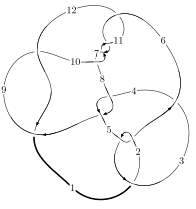
\includegraphics[width=112pt]{../../../GIT/diagram.site/Diagrams/png/2154_12n_0065.png}\\
\ \ \ A knot diagram\footnotemark}&
\allowdisplaybreaks
\textbf{Linearized knot diagam} \\
\cline{2-2}
 &
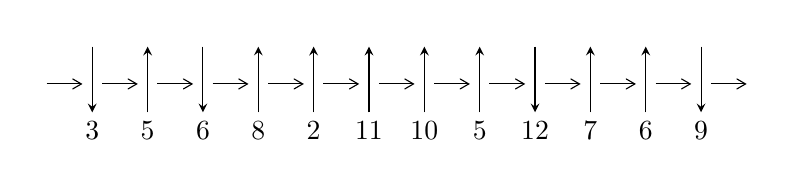
\begin{tikzpicture}[x=20pt, y=17pt]
	% nodes
	\node (C0) at (0, 0) {};
	\node (C1) at (1, 0) {};
	\node (C1U) at (1, +1) {};
	\node (C1D) at (1, -1) {3};

	\node (C2) at (2, 0) {};
	\node (C2U) at (2, +1) {};
	\node (C2D) at (2, -1) {5};

	\node (C3) at (3, 0) {};
	\node (C3U) at (3, +1) {};
	\node (C3D) at (3, -1) {6};

	\node (C4) at (4, 0) {};
	\node (C4U) at (4, +1) {};
	\node (C4D) at (4, -1) {8};

	\node (C5) at (5, 0) {};
	\node (C5U) at (5, +1) {};
	\node (C5D) at (5, -1) {2};

	\node (C6) at (6, 0) {};
	\node (C6U) at (6, +1) {};
	\node (C6D) at (6, -1) {11};

	\node (C7) at (7, 0) {};
	\node (C7U) at (7, +1) {};
	\node (C7D) at (7, -1) {10};

	\node (C8) at (8, 0) {};
	\node (C8U) at (8, +1) {};
	\node (C8D) at (8, -1) {5};

	\node (C9) at (9, 0) {};
	\node (C9U) at (9, +1) {};
	\node (C9D) at (9, -1) {12};

	\node (C10) at (10, 0) {};
	\node (C10U) at (10, +1) {};
	\node (C10D) at (10, -1) {7};

	\node (C11) at (11, 0) {};
	\node (C11U) at (11, +1) {};
	\node (C11D) at (11, -1) {6};

	\node (C12) at (12, 0) {};
	\node (C12U) at (12, +1) {};
	\node (C12D) at (12, -1) {9};
	\node (C13) at (13, 0) {};

	% arrows
	\draw[->,>={angle 60}]
	(C0) edge (C1) (C1) edge (C2) (C2) edge (C3) (C3) edge (C4) (C4) edge (C5) (C5) edge (C6) (C6) edge (C7) (C7) edge (C8) (C8) edge (C9) (C9) edge (C10) (C10) edge (C11) (C11) edge (C12) (C12) edge (C13) ;	\draw[->,>=stealth]
	(C1U) edge (C1D) (C2D) edge (C2U) (C3U) edge (C3D) (C4D) edge (C4U) (C5D) edge (C5U) (C6D) edge (C6U) (C7D) edge (C7U) (C8D) edge (C8U) (C9U) edge (C9D) (C10D) edge (C10U) (C11D) edge (C11U) (C12U) edge (C12D) ;
	\end{tikzpicture} \\
\hhline{~~} \\& 
\textbf{Solving Sequence} \\ \cline{2-2} 
 &
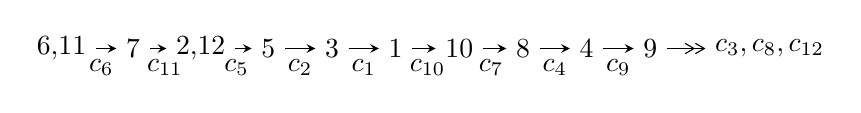
\begin{tikzpicture}[x=23pt, y=7pt]
	% node
	\node (A0) at (-1/8, 0) {6,11};
	\node (A1) at (1, 0) {7};
	\node (A2) at (33/16, 0) {2,12};
	\node (A3) at (25/8, 0) {5};
	\node (A4) at (33/8, 0) {3};
	\node (A5) at (41/8, 0) {1};
	\node (A6) at (49/8, 0) {10};
	\node (A7) at (57/8, 0) {8};
	\node (A8) at (65/8, 0) {4};
	\node (A9) at (73/8, 0) {9};
	\node (C1) at (1/2, -1) {$c_{6}$};
	\node (C2) at (3/2, -1) {$c_{11}$};
	\node (C3) at (21/8, -1) {$c_{5}$};
	\node (C4) at (29/8, -1) {$c_{2}$};
	\node (C5) at (37/8, -1) {$c_{1}$};
	\node (C6) at (45/8, -1) {$c_{10}$};
	\node (C7) at (53/8, -1) {$c_{7}$};
	\node (C8) at (61/8, -1) {$c_{4}$};
	\node (C9) at (69/8, -1) {$c_{9}$};
	\node (A10) at (11, 0) {$c_{3},c_{8},c_{12}$};

	% edge
	\draw[->,>=stealth]	
	(A0) edge (A1) (A1) edge (A2) (A2) edge (A3) (A3) edge (A4) (A4) edge (A5) (A5) edge (A6) (A6) edge (A7) (A7) edge (A8) (A8) edge (A9) ;
	\draw[->>,>={angle 60}]	
	(A9) edge (A10);
\end{tikzpicture} \\ 

\end{tabular} \\

\footnotetext{
The image of knot diagram is generated by the software ``\textbf{Draw programme}" developed by Andrew Bartholomew(\url{http://www.layer8.co.uk/maths/draw/index.htm\#Running-draw}), where we modified some parts for our purpose(\url{https://github.com/CATsTAILs/LinksPainter}).
}\phantom \\ \newline 
\centering \textbf{Ideals for irreducible components\footnotemark of $X_{\text{par}}$} 
 
\begin{align*}
I^u_{1}&=\langle 
- u^{22}+2 u^{21}+\cdots+2 b-2 u,\;-2 u^{22}+5 u^{21}+\cdots+2 a+4,\;u^{23}-3 u^{22}+\cdots-4 u+1\rangle \\
I^u_{2}&=\langle 
-4 u^3 a-2 u^2 a-4 u^3-11 a u-2 u^2+11 b-8 a-11 u-8,\\
\phantom{I^u_{2}}&\phantom{= \langle  }u^3 a+u^2 a- u^3+a^2+3 a u-2 u^2+2 a-4 u-2,\;u^4+u^3+3 u^2+2 u+1\rangle \\
\\
\end{align*}
\raggedright * 2 irreducible components of $\dim_{\mathbb{C}}=0$, with total 31 representations.\\
\footnotetext{All coefficients of polynomials are rational numbers. But the coefficients are sometimes approximated in decimal forms when there is not enough margin.}
\newpage
\renewcommand{\arraystretch}{1}
\centering \section*{I. $I^u_{1}= \langle - u^{22}+2 u^{21}+\cdots+2 b-2 u,\;-2 u^{22}+5 u^{21}+\cdots+2 a+4,\;u^{23}-3 u^{22}+\cdots-4 u+1 \rangle$}
\flushleft \textbf{(i) Arc colorings}\\
\begin{tabular}{m{7pt} m{180pt} m{7pt} m{180pt} }
\flushright $a_{6}=$&$\begin{pmatrix}1\\0\end{pmatrix}$ \\
\flushright $a_{11}=$&$\begin{pmatrix}0\\u\end{pmatrix}$ \\
\flushright $a_{7}=$&$\begin{pmatrix}1\\- u^2\end{pmatrix}$ \\
\flushright $a_{2}=$&$\begin{pmatrix}u^{22}-\frac{5}{2} u^{21}+\cdots-\frac{11}{2} u^2-2\\\frac{1}{2} u^{22}- u^{21}+\cdots+2 u^2+u\end{pmatrix}$ \\
\flushright $a_{12}=$&$\begin{pmatrix}u\\u\end{pmatrix}$ \\
\flushright $a_{5}=$&$\begin{pmatrix}-\frac{1}{2} u^{22}+\frac{3}{2} u^{21}+\cdots-7 u+2\\\frac{1}{2} u^{22}- u^{21}+\cdots+u-1\end{pmatrix}$ \\
\flushright $a_{3}=$&$\begin{pmatrix}-\frac{1}{2} u^{21}-4 u^{19}+\cdots-5 u+1\\\frac{3}{2} u^{22}-4 u^{21}+\cdots+4 u-2\end{pmatrix}$ \\
\flushright $a_{1}=$&$\begin{pmatrix}- u^9-4 u^7-3 u^5+2 u^3- u\\- u^9-5 u^7-7 u^5-2 u^3- u\end{pmatrix}$ \\
\flushright $a_{10}=$&$\begin{pmatrix}- u\\u^3+u\end{pmatrix}$ \\
\flushright $a_{8}=$&$\begin{pmatrix}u^2+1\\- u^4-2 u^2\end{pmatrix}$ \\
\flushright $a_{4}=$&$\begin{pmatrix}-\frac{3}{2} u^{22}+\frac{7}{2} u^{21}+\cdots-9 u+3\\\frac{3}{2} u^{22}-4 u^{21}+\cdots+4 u-2\end{pmatrix}$ \\
\flushright $a_{9}=$&$\begin{pmatrix}u^5+2 u^3- u\\u^5+3 u^3+u\end{pmatrix}$\\&\end{tabular}
\flushleft \textbf{(ii) Obstruction class $= -1$}\\~\\
\flushleft \textbf{(iii) Cusp Shapes $= -\frac{3}{2} u^{22}+3 u^{21}-21 u^{20}+\frac{73}{2} u^{19}-124 u^{18}+186 u^{17}-400 u^{16}+506 u^{15}-\frac{1519}{2} u^{14}+\frac{1537}{2} u^{13}-845 u^{12}+605 u^{11}-\frac{1015}{2} u^{10}+178 u^9-\frac{265}{2} u^8-\frac{33}{2} u^7-\frac{29}{2} u^6-\frac{67}{2} u^5-\frac{5}{2} u^4-49 u^3+\frac{19}{2} u^2+\frac{7}{2}$}\\~\\
\newpage\renewcommand{\arraystretch}{1}
\flushleft \textbf{(iv) u-Polynomials at the component}\newline \\
\begin{tabular}{m{50pt}|m{274pt}}
Crossings & \hspace{64pt}u-Polynomials at each crossing \\
\hline $$\begin{aligned}c_{1}\end{aligned}$$&$\begin{aligned}
&u^{23}+3 u^{22}+\cdots+4 u-1
\end{aligned}$\\
\hline $$\begin{aligned}c_{2},c_{5}\end{aligned}$$&$\begin{aligned}
&u^{23}+5 u^{22}+\cdots-4 u-1
\end{aligned}$\\
\hline $$\begin{aligned}c_{3}\end{aligned}$$&$\begin{aligned}
&u^{23}-5 u^{22}+\cdots-2678 u-593
\end{aligned}$\\
\hline $$\begin{aligned}c_{4},c_{8}\end{aligned}$$&$\begin{aligned}
&u^{23}- u^{22}+\cdots+128 u-256
\end{aligned}$\\
\hline $$\begin{aligned}c_{6},c_{7},c_{10}\\c_{11}\end{aligned}$$&$\begin{aligned}
&u^{23}+3 u^{22}+\cdots-4 u-1
\end{aligned}$\\
\hline $$\begin{aligned}c_{9},c_{12}\end{aligned}$$&$\begin{aligned}
&u^{23}- u^{22}+\cdots+2 u^2-1
\end{aligned}$\\
\hline
\end{tabular}\\~\\
\newpage\renewcommand{\arraystretch}{1}
\flushleft \textbf{(v) Riley Polynomials at the component}\newline \\
\begin{tabular}{m{50pt}|m{274pt}}
Crossings & \hspace{64pt}Riley Polynomials at each crossing \\
\hline $$\begin{aligned}c_{1}\end{aligned}$$&$\begin{aligned}
&y^{23}+39 y^{22}+\cdots+4 y-1
\end{aligned}$\\
\hline $$\begin{aligned}c_{2},c_{5}\end{aligned}$$&$\begin{aligned}
&y^{23}+3 y^{22}+\cdots+4 y-1
\end{aligned}$\\
\hline $$\begin{aligned}c_{3}\end{aligned}$$&$\begin{aligned}
&y^{23}+75 y^{22}+\cdots-15091908 y-351649
\end{aligned}$\\
\hline $$\begin{aligned}c_{4},c_{8}\end{aligned}$$&$\begin{aligned}
&y^{23}-45 y^{22}+\cdots-212992 y-65536
\end{aligned}$\\
\hline $$\begin{aligned}c_{6},c_{7},c_{10}\\c_{11}\end{aligned}$$&$\begin{aligned}
&y^{23}+25 y^{22}+\cdots+4 y-1
\end{aligned}$\\
\hline $$\begin{aligned}c_{9},c_{12}\end{aligned}$$&$\begin{aligned}
&y^{23}+41 y^{22}+\cdots+4 y-1
\end{aligned}$\\
\hline
\end{tabular}\\~\\
\newpage\flushleft \textbf{(vi) Complex Volumes and Cusp Shapes}
$$\begin{array}{c|c|c}  
\text{Solutions to }I^u_{1}& \I (\text{vol} + \sqrt{-1}CS) & \text{Cusp shape}\\
 \hline 
\begin{aligned}
u &= \phantom{-}0.768656 + 0.574390 I \\
a &= \phantom{-}0.96411 - 1.30127 I \\
b &= -1.02013 - 1.06010 I\end{aligned}
 & \phantom{-}14.5386 + 6.4049 I & \phantom{-}5.87992 - 4.56999 I \\ \hline\begin{aligned}
u &= \phantom{-}0.768656 - 0.574390 I \\
a &= \phantom{-}0.96411 + 1.30127 I \\
b &= -1.02013 + 1.06010 I\end{aligned}
 & \phantom{-}14.5386 - 6.4049 I & \phantom{-}5.87992 + 4.56999 I \\ \hline\begin{aligned}
u &= \phantom{-}0.792664 + 0.509239 I \\
a &= -0.193691 - 0.034587 I \\
b &= -1.06482 + 1.00488 I\end{aligned}
 & \phantom{-}14.7384 - 1.2262 I & \phantom{-}6.30437 - 0.37163 I \\ \hline\begin{aligned}
u &= \phantom{-}0.792664 - 0.509239 I \\
a &= -0.193691 + 0.034587 I \\
b &= -1.06482 - 1.00488 I\end{aligned}
 & \phantom{-}14.7384 + 1.2262 I & \phantom{-}6.30437 + 0.37163 I \\ \hline\begin{aligned}
u &= -0.502322 + 0.520642 I \\
a &= \phantom{-}0.811150 + 0.610068 I \\
b &= -0.461371 + 0.176461 I\end{aligned}
 & \phantom{-}0.70832 - 1.75933 I & \phantom{-}4.65925 + 3.45911 I \\ \hline\begin{aligned}
u &= -0.502322 - 0.520642 I \\
a &= \phantom{-}0.811150 - 0.610068 I \\
b &= -0.461371 - 0.176461 I\end{aligned}
 & \phantom{-}0.70832 + 1.75933 I & \phantom{-}4.65925 - 3.45911 I \\ \hline\begin{aligned}
u &= -0.038925 + 1.309910 I \\
a &= \phantom{-}0.467966 - 0.365892 I \\
b &= \phantom{-}0.881690 - 0.526981 I\end{aligned}
 & -2.62006 - 1.64777 I & \phantom{-}3.52749 + 2.17174 I \\ \hline\begin{aligned}
u &= -0.038925 - 1.309910 I \\
a &= \phantom{-}0.467966 + 0.365892 I \\
b &= \phantom{-}0.881690 + 0.526981 I\end{aligned}
 & -2.62006 + 1.64777 I & \phantom{-}3.52749 - 2.17174 I \\ \hline\begin{aligned}
u &= \phantom{-}0.091640 + 1.402330 I \\
a &= -0.60254 + 2.18385 I \\
b &= \phantom{-}0.586427 + 1.117770 I\end{aligned}
 & -4.58949 + 3.87928 I & \phantom{-}1.77141 - 2.75540 I \\ \hline\begin{aligned}
u &= \phantom{-}0.091640 - 1.402330 I \\
a &= -0.60254 - 2.18385 I \\
b &= \phantom{-}0.586427 - 1.117770 I\end{aligned}
 & -4.58949 - 3.87928 I & \phantom{-}1.77141 + 2.75540 I\\
 \hline 
 \end{array}$$\newpage$$\begin{array}{c|c|c}  
\text{Solutions to }I^u_{1}& \I (\text{vol} + \sqrt{-1}CS) & \text{Cusp shape}\\
 \hline 
\begin{aligned}
u &= -0.091228 + 0.543350 I \\
a &= \phantom{-}1.15824 - 1.74645 I \\
b &= \phantom{-}0.243917 - 0.711016 I\end{aligned}
 & -1.17938 - 1.49722 I & -2.53958 + 5.27560 I \\ \hline\begin{aligned}
u &= -0.091228 - 0.543350 I \\
a &= \phantom{-}1.15824 + 1.74645 I \\
b &= \phantom{-}0.243917 + 0.711016 I\end{aligned}
 & -1.17938 + 1.49722 I & -2.53958 - 5.27560 I \\ \hline\begin{aligned}
u &= -0.464696\phantom{ +0.000000I} \\
a &= \phantom{-}0.105740\phantom{ +0.000000I} \\
b &= \phantom{-}0.580286\phantom{ +0.000000I}\end{aligned}
 & \phantom{-}1.11404\phantom{ +0.000000I} & \phantom{-}10.0250\phantom{ +0.000000I} \\ \hline\begin{aligned}
u &= -0.05085 + 1.53575 I \\
a &= \phantom{-}0.55421 - 2.04140 I \\
b &= \phantom{-}0.003120 - 0.853741 I\end{aligned}
 & -8.14932 - 2.13339 I & -3.53476 + 3.27759 I \\ \hline\begin{aligned}
u &= -0.05085 - 1.53575 I \\
a &= \phantom{-}0.55421 + 2.04140 I \\
b &= \phantom{-}0.003120 + 0.853741 I\end{aligned}
 & -8.14932 + 2.13339 I & -3.53476 - 3.27759 I \\ \hline\begin{aligned}
u &= \phantom{-}0.29102 + 1.52358 I \\
a &= -1.009020 + 0.577805 I \\
b &= -1.08811 + 0.92523 I\end{aligned}
 & \phantom{-}8.14473 + 2.74909 I & \phantom{-}3.44638 - 0.72919 I \\ \hline\begin{aligned}
u &= \phantom{-}0.29102 - 1.52358 I \\
a &= -1.009020 - 0.577805 I \\
b &= -1.08811 - 0.92523 I\end{aligned}
 & \phantom{-}8.14473 - 2.74909 I & \phantom{-}3.44638 + 0.72919 I \\ \hline\begin{aligned}
u &= -0.13755 + 1.55696 I \\
a &= \phantom{-}0.363925 + 1.080750 I \\
b &= -0.509748 + 0.419465 I\end{aligned}
 & -6.30985 - 4.03193 I & \phantom{-}1.37603 + 1.02672 I \\ \hline\begin{aligned}
u &= -0.13755 - 1.55696 I \\
a &= \phantom{-}0.363925 - 1.080750 I \\
b &= -0.509748 - 0.419465 I\end{aligned}
 & -6.30985 + 4.03193 I & \phantom{-}1.37603 - 1.02672 I \\ \hline\begin{aligned}
u &= \phantom{-}0.26608 + 1.55802 I \\
a &= \phantom{-}0.27719 - 2.09273 I \\
b &= -0.96060 - 1.09404 I\end{aligned}
 & \phantom{-}7.54756 + 10.22760 I & \phantom{-}2.79101 - 4.77678 I\\
 \hline 
 \end{array}$$\newpage$$\begin{array}{c|c|c}  
\text{Solutions to }I^u_{1}& \I (\text{vol} + \sqrt{-1}CS) & \text{Cusp shape}\\
 \hline 
\begin{aligned}
u &= \phantom{-}0.26608 - 1.55802 I \\
a &= \phantom{-}0.27719 + 2.09273 I \\
b &= -0.96060 + 1.09404 I\end{aligned}
 & \phantom{-}7.54756 - 10.22760 I & \phantom{-}2.79101 + 4.77678 I \\ \hline\begin{aligned}
u &= \phantom{-}0.343175 + 0.152187 I \\
a &= -2.34441 + 0.12809 I \\
b &= \phantom{-}0.599485 + 0.898495 I\end{aligned}
 & \phantom{-}0.46499 + 2.40467 I & \phantom{-}3.80616 - 1.75250 I \\ \hline\begin{aligned}
u &= \phantom{-}0.343175 - 0.152187 I \\
a &= -2.34441 - 0.12809 I \\
b &= \phantom{-}0.599485 - 0.898495 I\end{aligned}
 & \phantom{-}0.46499 - 2.40467 I & \phantom{-}3.80616 + 1.75250 I\\
 \hline 
 \end{array}$$\newpage\newpage\renewcommand{\arraystretch}{1}
\centering \section*{II. $I^u_{2}= \langle -4 u^3 a-4 u^3+\cdots-8 a-8,\;u^3 a- u^3+\cdots+2 a-2,\;u^4+u^3+3 u^2+2 u+1 \rangle$}
\flushleft \textbf{(i) Arc colorings}\\
\begin{tabular}{m{7pt} m{180pt} m{7pt} m{180pt} }
\flushright $a_{6}=$&$\begin{pmatrix}1\\0\end{pmatrix}$ \\
\flushright $a_{11}=$&$\begin{pmatrix}0\\u\end{pmatrix}$ \\
\flushright $a_{7}=$&$\begin{pmatrix}1\\- u^2\end{pmatrix}$ \\
\flushright $a_{2}=$&$\begin{pmatrix}a\\0.363636 a u^{3}+0.363636 u^{3}+\cdots+0.727273 a+0.727273\end{pmatrix}$ \\
\flushright $a_{12}=$&$\begin{pmatrix}u\\u\end{pmatrix}$ \\
\flushright $a_{5}=$&$\begin{pmatrix}-0.363636 a u^{3}+0.636364 u^{3}+\cdots+0.272727 a+1.27273\\0.363636 a u^{3}+0.363636 u^{3}+\cdots+0.727273 a-0.272727\end{pmatrix}$ \\
\flushright $a_{3}=$&$\begin{pmatrix}u^3+u^2+a+3 u+1\\0.363636 a u^{3}+0.363636 u^{3}+\cdots+0.727273 a-0.272727\end{pmatrix}$ \\
\flushright $a_{1}=$&$\begin{pmatrix}-1\\0\end{pmatrix}$ \\
\flushright $a_{10}=$&$\begin{pmatrix}- u\\u^3+u\end{pmatrix}$ \\
\flushright $a_{8}=$&$\begin{pmatrix}u^2+1\\u^3+u^2+2 u+1\end{pmatrix}$ \\
\flushright $a_{4}=$&$\begin{pmatrix}-0.363636 a u^{3}+0.636364 u^{3}+\cdots+0.272727 a+1.27273\\0.363636 a u^{3}+0.363636 u^{3}+\cdots+0.727273 a-0.272727\end{pmatrix}$ \\
\flushright $a_{9}=$&$\begin{pmatrix}u^2+1\\u^3+u^2+2 u+1\end{pmatrix}$\\&\end{tabular}
\flushleft \textbf{(ii) Obstruction class $= 1$}\\~\\
\flushleft \textbf{(iii) Cusp Shapes $= -2 u^3 a- u^2 a+2 u^3-6 a u+3 u^2-3 a+7 u+7$}\\~\\
\newpage\renewcommand{\arraystretch}{1}
\flushleft \textbf{(iv) u-Polynomials at the component}\newline \\
\begin{tabular}{m{50pt}|m{274pt}}
Crossings & \hspace{64pt}u-Polynomials at each crossing \\
\hline $$\begin{aligned}c_{1},c_{3},c_{5}\end{aligned}$$&$\begin{aligned}
&(u^2- u+1)^4
\end{aligned}$\\
\hline $$\begin{aligned}c_{2}\end{aligned}$$&$\begin{aligned}
&(u^2+u+1)^4
\end{aligned}$\\
\hline $$\begin{aligned}c_{4},c_{8}\end{aligned}$$&$\begin{aligned}
&u^8
\end{aligned}$\\
\hline $$\begin{aligned}c_{6},c_{7}\end{aligned}$$&$\begin{aligned}
&(u^4+u^3+3 u^2+2 u+1)^2
\end{aligned}$\\
\hline $$\begin{aligned}c_{9}\end{aligned}$$&$\begin{aligned}
&(u^4+u^3+u^2+1)^2
\end{aligned}$\\
\hline $$\begin{aligned}c_{10},c_{11}\end{aligned}$$&$\begin{aligned}
&(u^4- u^3+3 u^2-2 u+1)^2
\end{aligned}$\\
\hline $$\begin{aligned}c_{12}\end{aligned}$$&$\begin{aligned}
&(u^4- u^3+u^2+1)^2
\end{aligned}$\\
\hline
\end{tabular}\\~\\
\newpage\renewcommand{\arraystretch}{1}
\flushleft \textbf{(v) Riley Polynomials at the component}\newline \\
\begin{tabular}{m{50pt}|m{274pt}}
Crossings & \hspace{64pt}Riley Polynomials at each crossing \\
\hline $$\begin{aligned}c_{1},c_{2},c_{3}\\c_{5}\end{aligned}$$&$\begin{aligned}
&(y^2+y+1)^4
\end{aligned}$\\
\hline $$\begin{aligned}c_{4},c_{8}\end{aligned}$$&$\begin{aligned}
&y^8
\end{aligned}$\\
\hline $$\begin{aligned}c_{6},c_{7},c_{10}\\c_{11}\end{aligned}$$&$\begin{aligned}
&(y^4+5 y^3+7 y^2+2 y+1)^2
\end{aligned}$\\
\hline $$\begin{aligned}c_{9},c_{12}\end{aligned}$$&$\begin{aligned}
&(y^4+y^3+3 y^2+2 y+1)^2
\end{aligned}$\\
\hline
\end{tabular}\\~\\
\newpage\flushleft \textbf{(vi) Complex Volumes and Cusp Shapes}
$$\begin{array}{c|c|c}  
\text{Solutions to }I^u_{2}& \I (\text{vol} + \sqrt{-1}CS) & \text{Cusp shape}\\
 \hline 
\begin{aligned}
u &= -0.395123 + 0.506844 I \\
a &= \phantom{-}0.584432 + 0.289945 I \\
b &= \phantom{-}0.500000 + 0.866025 I\end{aligned}
 & \phantom{-}0.211005 + 0.614778 I & \phantom{-}4.65255 + 0.59814 I \\ \hline\begin{aligned}
u &= -0.395123 + 0.506844 I \\
a &= -1.54112 - 1.51713 I \\
b &= \phantom{-}0.500000 - 0.866025 I\end{aligned}
 & \phantom{-}0.21101 - 3.44499 I & \phantom{-}1.64912 + 8.49900 I \\ \hline\begin{aligned}
u &= -0.395123 - 0.506844 I \\
a &= \phantom{-}0.584432 - 0.289945 I \\
b &= \phantom{-}0.500000 - 0.866025 I\end{aligned}
 & \phantom{-}0.211005 - 0.614778 I & \phantom{-}4.65255 - 0.59814 I \\ \hline\begin{aligned}
u &= -0.395123 - 0.506844 I \\
a &= -1.54112 + 1.51713 I \\
b &= \phantom{-}0.500000 + 0.866025 I\end{aligned}
 & \phantom{-}0.21101 + 3.44499 I & \phantom{-}1.64912 - 8.49900 I \\ \hline\begin{aligned}
u &= -0.10488 + 1.55249 I \\
a &= \phantom{-}0.53364 + 1.37394 I \\
b &= \phantom{-}0.500000 + 0.866025 I\end{aligned}
 & -6.79074 - 1.13408 I & \phantom{-}1.99896 - 0.39034 I \\ \hline\begin{aligned}
u &= -0.10488 + 1.55249 I \\
a &= -0.57695 - 2.01514 I \\
b &= \phantom{-}0.500000 - 0.866025 I\end{aligned}
 & -6.79074 - 5.19385 I & -1.80063 + 6.43123 I \\ \hline\begin{aligned}
u &= -0.10488 - 1.55249 I \\
a &= \phantom{-}0.53364 - 1.37394 I \\
b &= \phantom{-}0.500000 - 0.866025 I\end{aligned}
 & -6.79074 + 1.13408 I & \phantom{-}1.99896 + 0.39034 I \\ \hline\begin{aligned}
u &= -0.10488 - 1.55249 I \\
a &= -0.57695 + 2.01514 I \\
b &= \phantom{-}0.500000 + 0.866025 I\end{aligned}
 & -6.79074 + 5.19385 I & -1.80063 - 6.43123 I\\
 \hline 
 \end{array}$$\newpage
\newpage\renewcommand{\arraystretch}{1}
\centering \section*{ III. u-Polynomials}
\begin{tabular}{m{50pt}|m{274pt}}
Crossings & \hspace{64pt}u-Polynomials at each crossing \\
\hline $$\begin{aligned}c_{1}\end{aligned}$$&$\begin{aligned}
&((u^2- u+1)^4)(u^{23}+3 u^{22}+\cdots+4 u-1)
\end{aligned}$\\
\hline $$\begin{aligned}c_{2}\end{aligned}$$&$\begin{aligned}
&((u^2+u+1)^4)(u^{23}+5 u^{22}+\cdots-4 u-1)
\end{aligned}$\\
\hline $$\begin{aligned}c_{3}\end{aligned}$$&$\begin{aligned}
&((u^2- u+1)^4)(u^{23}-5 u^{22}+\cdots-2678 u-593)
\end{aligned}$\\
\hline $$\begin{aligned}c_{4},c_{8}\end{aligned}$$&$\begin{aligned}
&u^8(u^{23}- u^{22}+\cdots+128 u-256)
\end{aligned}$\\
\hline $$\begin{aligned}c_{5}\end{aligned}$$&$\begin{aligned}
&((u^2- u+1)^4)(u^{23}+5 u^{22}+\cdots-4 u-1)
\end{aligned}$\\
\hline $$\begin{aligned}c_{6},c_{7}\end{aligned}$$&$\begin{aligned}
&((u^4+u^3+3 u^2+2 u+1)^2)(u^{23}+3 u^{22}+\cdots-4 u-1)
\end{aligned}$\\
\hline $$\begin{aligned}c_{9}\end{aligned}$$&$\begin{aligned}
&((u^4+u^3+u^2+1)^2)(u^{23}- u^{22}+\cdots+2 u^2-1)
\end{aligned}$\\
\hline $$\begin{aligned}c_{10},c_{11}\end{aligned}$$&$\begin{aligned}
&((u^4- u^3+3 u^2-2 u+1)^2)(u^{23}+3 u^{22}+\cdots-4 u-1)
\end{aligned}$\\
\hline $$\begin{aligned}c_{12}\end{aligned}$$&$\begin{aligned}
&((u^4- u^3+u^2+1)^2)(u^{23}- u^{22}+\cdots+2 u^2-1)
\end{aligned}$\\
\hline
\end{tabular}\newpage\renewcommand{\arraystretch}{1}
\centering \section*{ IV. Riley Polynomials}
\begin{tabular}{m{50pt}|m{274pt}}
Crossings & \hspace{64pt}Riley Polynomials at each crossing \\
\hline $$\begin{aligned}c_{1}\end{aligned}$$&$\begin{aligned}
&((y^2+y+1)^4)(y^{23}+39 y^{22}+\cdots+4 y-1)
\end{aligned}$\\
\hline $$\begin{aligned}c_{2},c_{5}\end{aligned}$$&$\begin{aligned}
&((y^2+y+1)^4)(y^{23}+3 y^{22}+\cdots+4 y-1)
\end{aligned}$\\
\hline $$\begin{aligned}c_{3}\end{aligned}$$&$\begin{aligned}
&((y^2+y+1)^4)(y^{23}+75 y^{22}+\cdots-1.50919\times10^{7} y-351649)
\end{aligned}$\\
\hline $$\begin{aligned}c_{4},c_{8}\end{aligned}$$&$\begin{aligned}
&y^8(y^{23}-45 y^{22}+\cdots-212992 y-65536)
\end{aligned}$\\
\hline $$\begin{aligned}c_{6},c_{7},c_{10}\\c_{11}\end{aligned}$$&$\begin{aligned}
&((y^4+5 y^3+7 y^2+2 y+1)^2)(y^{23}+25 y^{22}+\cdots+4 y-1)
\end{aligned}$\\
\hline $$\begin{aligned}c_{9},c_{12}\end{aligned}$$&$\begin{aligned}
&((y^4+y^3+3 y^2+2 y+1)^2)(y^{23}+41 y^{22}+\cdots+4 y-1)
\end{aligned}$\\
\hline
\end{tabular}
\vskip 2pc
\end{document}